 \documentclass{report}
\usepackage[utf8]{inputenc}
\setlength{\parindent}{0.5em}
\setlength{\parskip}{0.5em}
\usepackage{pgfplots}
\usepackage{circuitikz}
\usepackage{verbatim}
\usepackage{graphicx}
\usepackage{siunitx}
\pgfplotsset{width=7cm,compat=1.8}
\graphicspath{{./work/}}
\title{Report}
\usepackage{polyglossia}
\author{Diluna Adeesha Warnakulasuriya}
\date{\today}

\begin{document}

\maketitle
\chapter{Theoretical Part}
\begin{center}
    

\begin{circuitikz} 
\draw
(0,4) to[battery=$V_1$] (0,0)
  to (4,0)
  to[resistor=$R_2$]  (4,4)
  to [resistor=$R_1$] (0,4)
;
\end{circuitikz}\newline
\hfill \break
\begin{tikzpicture}
  \begin{axis}[
  height=9cm,
		width=9cm,
		grid=both,
		tick align=inside,
		minor tick num=3,
		major tick style={black,thin},
		minor tick style={black},
		major grid style={color=gray!60,densely dashed},
		minor grid style={color=gray!50,densely dotted},
		tick label style={font=\footnotesize},
		label style={font=\normalsize},
		xlabel=$f(R2)$,
		ylabel=$U(R2)$,
		title={U(R2) = f(R2)}]
    \addplot+[smooth] coordinates {
		(5, 0.583) +- (10, 0.636)
		(15, 0.656) +- (20, 0.667)
		(25, 0.673) +- (30, 0.677)
		(35, 0.681) +- (40, 0.683)
		(45, 0.685) +- (50, 0.686)};
	\end{axis}
\end{tikzpicture}
\end{center}

\section{Circuit calculation}
Calculated the Voltages on the Resistors R1 and R2 in DC circuit using Voltage Division Rule.

\[V_{R1} =(V_{1} \times R_{1})/(R_{1} + R_{2})
\]
\[V_{R2} =(V_{1} \times R_{2})/(R_{1} + R_{2})
\]
\hfill \break

 
\begin{figure}[h]

\begin{center}
\begin{math} 
\begin{tabular}{|c|c|}
      \hline
     Variable & Value\\
    \hline
     R_{1}                   &  1\si{\ohm}\\
     \hline
     R_{2}  &  1\si{\ohm}\\
      \hline
     V_{1}  &  0.7V\\
      \hline
     V_{R2}  &  0.35V\\
      \hline
     V_{R1}  &  0.35V\\
     \hline
\end{tabular}
\end{math}
\caption{Table}
\end{center}
\end{figure}

\newpage
\chapter{Practicle Part}
\section{Work with GEDA programs}
\subsection{Work with gschem}
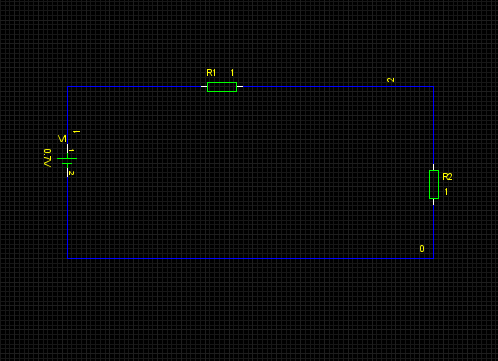
\includegraphics[]{schematics.png}
\subsection{Work with gnetlist}
\input{01.net}
\clearpage
\newpage
\subsection{Work with ngspice}
This is the picture i got from plotting Connectin "1"
\begin{figure}[h]
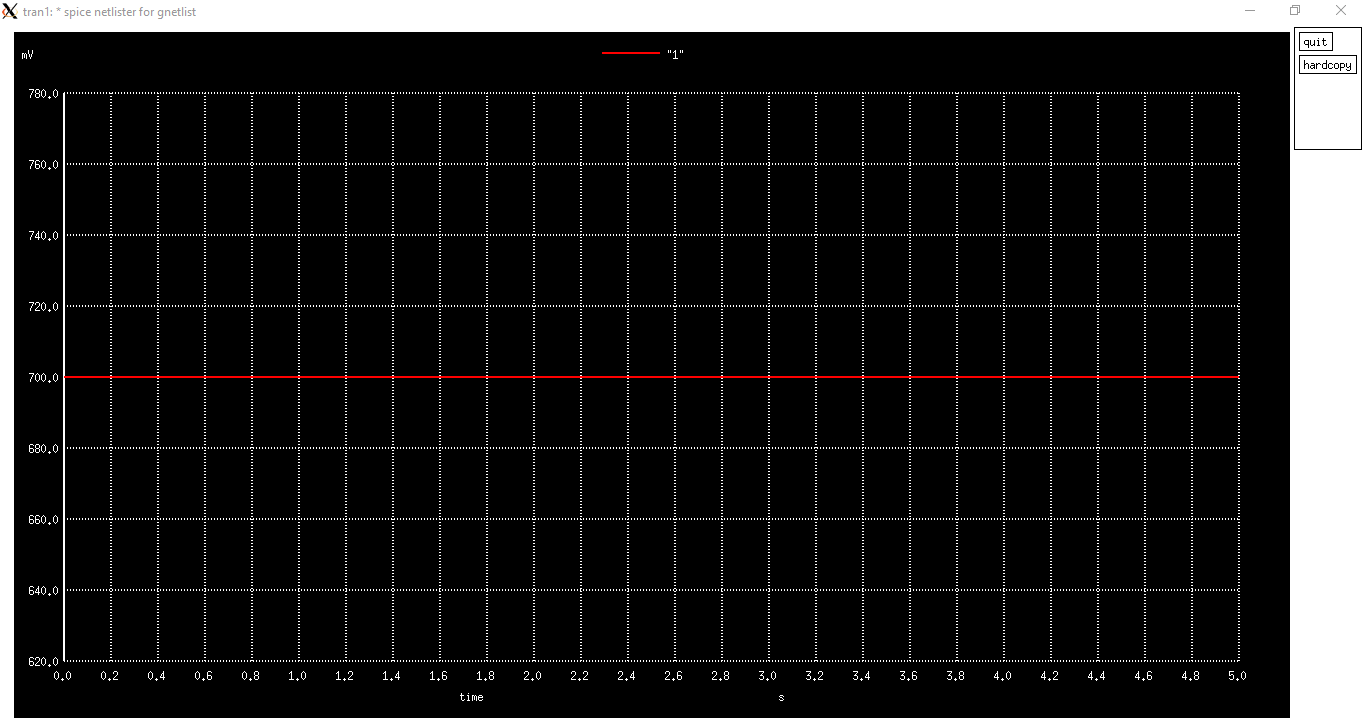
\includegraphics[scale=0.45]{011.png}
\newline
\centering
\caption{011.png}
\end{figure}
\newpage
This is the picture i got from plotting Connectin "2"
\begin{figure}[h]
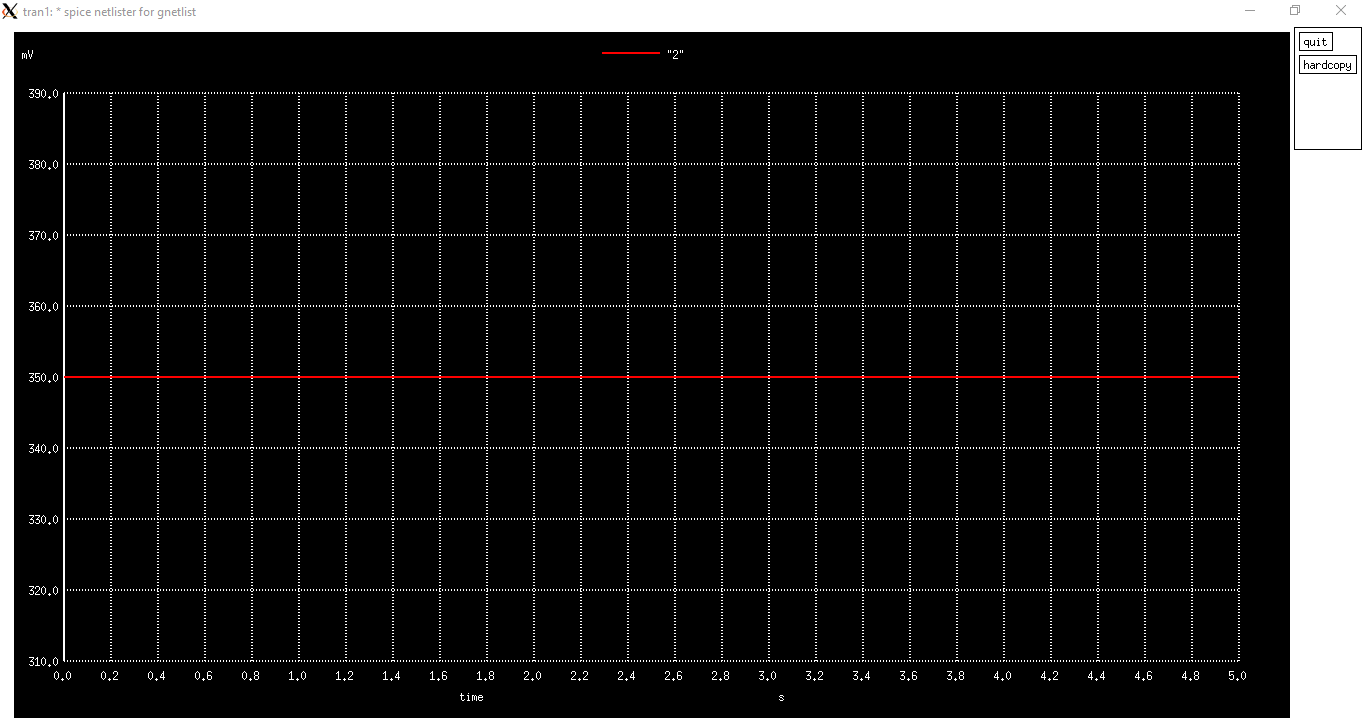
\includegraphics[scale=0.45]{012.png}
\newline
\caption{012.png}
\centering
\end{figure}
\newpage
\section{work with QUCS programs}
I setup a circuit with a graphical user interface (GUI) and simulate the DC signal and noise behaviour of the circuit. After that simulation has finished i viewed the simulation results on a presentation window.\hfill \break
\begin{figure}[h]
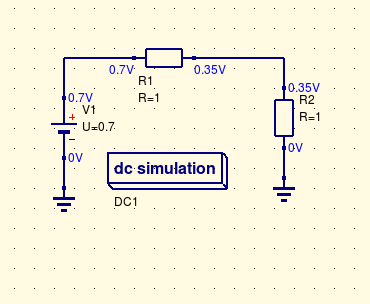
\includegraphics[]{02sch.png}
\newline
\centering
\caption{The QUCS schematics environment}
\end{figure}
\begin{itemize}
\item Perform elementary DC mode simulation with the F8 key, which results in calculations
and determines the voltage on the resistor R2.\newline
\hfill \break
\item It is shown in the image as 0.35V.\newline
\hfill \break
\item The simulator variable that derives this
value is designated R2.V.
\end{itemize}
\clearpage
\begin{figure}[h]
\centering
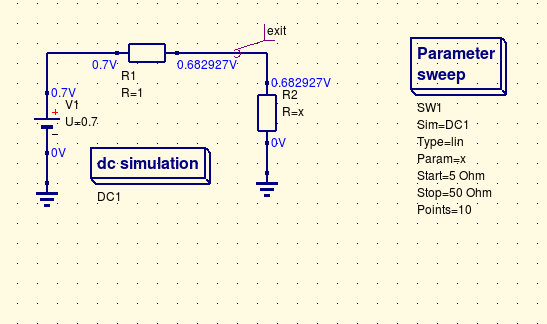
\includegraphics[]{03sch.png}
\caption{Parameter sweep mode}
\end{figure}
\begin{itemize}
\item the value of resistor R2 to the symbol x, which will serve as the argument for the
current circuit calculation.\newline symbol: x has also written in the Param field of the
component ‘parameter sweep’ attribute field.\newline
\hfill \break
\item Changed the number of points to 10. simulating parameter x  changed linearly\newline
\hfill \break
\item value 5 Ω to 50Ω at eleven points, where all the parameters of the circuit (current
and voltages)calculated corresponding number of times because they depend on
resistor R2 value.\newline
\hfill \break
\item the resulting parameter selection form, we can change them, obtain and estimate
the calculated voltage value on the resistor R2-UR2
\end{itemize}
\clearpage
\begin{figure}[h]
\centering
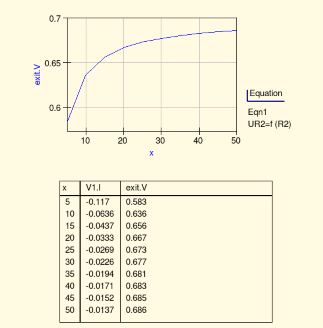
\includegraphics[]{02dpi.png}
\caption{Curve and Table from Sweep simulation}
\end{figure}
\begin{itemize}

\item This graph showing the
functional relationship between the value of R2 (which is variable) and the voltage on it -
UR2. Generally it can be write as ‘UR2 = f (R2)’.\newline
\hfill \break
\item The table
display the current (V1.I) flowing through the voltage source V1 and the electrical circuit
point with the signal output voltage (output V) against ”Ground” as a function of parameter
x.
\end{itemize}
\newpage
\section{Refferences}
\begin{itemize}
\item gschem to pcb tutorial, by Bill Wilson (release notes).\newline
\hfill \break
\item gschem warmup, by Bill Willson.\newline
\hfill \break
\item Mustafa Baser, “Effects of Conceptual Change and Traditional Confirmatory Simulations on Pre-Service Teachers’ Understanding of Direct Current Circuits”, Journal of Science Education and Technology, vol. 15, no. 5-6, Dec. 2006. Link: http://dx.doi.org/10.1007/s10956-006-9025-3.
\end{itemize}
\end{document}

